% =============================================================================
% COPYRIGHT AND DISCLAIMER
% =============================================================================
% This file is provided as a convenience template for competition participants.
% By using it, you accept full responsibility for compliance with all applicable
% copyright, licensing, and usage rules of the Association for Computing
% Machinery (ACM) and of any LaTeX packages you load (including, without
% limitation, the "acmart" document class and related ACM materials).
%
% Consult ACM's official publication, template, and copyright policies before
% using this setup for any purpose other than this competition. Do not assume
% that this template may be reused, redistributed, or submitted elsewhere
% without independently verifying ACM's current rules.
%
% Use of the "acmart" class, the "sigconf" option, or ACM-style formatting in
% this template does NOT mean that this report, this competition, its organizers,
% or any resulting PDF is sponsored, endorsed, affiliated with, or published by
% ACM. ACM trademarks and branding remain the property of ACM.
%
% Template packages live in preamble.tex.
% Citations live in main.bib. Edit this file with your paper content.
% =============================================================================

\documentclass[sigconf]{acmart}
% =============================================================================
% Template setup — participants normally do not edit this file.
% Author content belongs in main.tex; citations belong in main.bib.
% \documentclass lives in main.tex so Overleaf does not treat this file as root.
% =============================================================================

% --- Competition / non-ACM-submission friendly rights metadata -------------
\setcopyright{none}
\settopmatter{printacmref=false}
\acmConference[Kaggle Competition]{Filament Segmentation Challenge}{2026}{\href{https://www.kaggle.com/competitions/filament-segmentation-2026}{kaggle.com/competitions/filament-segmentation-2026}}
\acmBooktitle{Competition Report}
\acmDOI{}
\acmISBN{}

% --- Author guidance text --------------------------------------------------
% \guide{...} is gray italic while \guideStyletrue; omitted from the PDF if false.
% Flip the switch in main.tex after % =============================================================================
% Template setup — participants normally do not edit this file.
% Author content belongs in main.tex; citations belong in main.bib.
% \documentclass lives in main.tex so Overleaf does not treat this file as root.
% =============================================================================

% --- Competition / non-ACM-submission friendly rights metadata -------------
\setcopyright{none}
\settopmatter{printacmref=false}
\acmConference[Kaggle Competition]{Filament Segmentation Challenge}{2026}{\href{https://www.kaggle.com/competitions/filament-segmentation-2026}{kaggle.com/competitions/filament-segmentation-2026}}
\acmBooktitle{Competition Report}
\acmDOI{}
\acmISBN{}

% --- Author guidance text --------------------------------------------------
% \guide{...} is gray italic while \guideStyletrue; omitted from the PDF if false.
% Flip the switch in main.tex after % =============================================================================
% Template setup — participants normally do not edit this file.
% Author content belongs in main.tex; citations belong in main.bib.
% \documentclass lives in main.tex so Overleaf does not treat this file as root.
% =============================================================================

% --- Competition / non-ACM-submission friendly rights metadata -------------
\setcopyright{none}
\settopmatter{printacmref=false}
\acmConference[Kaggle Competition]{Filament Segmentation Challenge}{2026}{\href{https://www.kaggle.com/competitions/filament-segmentation-2026}{kaggle.com/competitions/filament-segmentation-2026}}
\acmBooktitle{Competition Report}
\acmDOI{}
\acmISBN{}

% --- Author guidance text --------------------------------------------------
% \guide{...} is gray italic while \guideStyletrue; omitted from the PDF if false.
% Flip the switch in main.tex after \input{preamble}.
%
% Do not use \guide{...} for \email{...}.
\usepackage{xcolor}
\newif\ifguideStyle
\guideStyletrue
\newcommand{\guide}[1]{%
  \ifguideStyle
    {\color{gray!65}\itshape #1}%
  \fi
}

% --- Math ------------------------------------------------------------------
% Do NOT load amssymb (or amsfonts): acmart already loads newtxmath, which
% defines the same symbols (e.g. \Bbbk) and causes a conflict on Overleaf.
% amsmath is already provided by acmart; mathtools extends it.
\usepackage{mathtools}

% --- Figures ---------------------------------------------------------------
% graphicx is already loaded by acmart
\usepackage{subcaption}

% --- Tables ----------------------------------------------------------------
% booktabs is already loaded by acmart
\usepackage{tabularx}
\usepackage{multirow}

% --- Bibliography style is set in main.tex (ACM-Reference-Format) ----------
.
%
% Do not use \guide{...} for \email{...}.
\usepackage{xcolor}
\newif\ifguideStyle
\guideStyletrue
\newcommand{\guide}[1]{%
  \ifguideStyle
    {\color{gray!65}\itshape #1}%
  \fi
}

% --- Math ------------------------------------------------------------------
% Do NOT load amssymb (or amsfonts): acmart already loads newtxmath, which
% defines the same symbols (e.g. \Bbbk) and causes a conflict on Overleaf.
% amsmath is already provided by acmart; mathtools extends it.
\usepackage{mathtools}

% --- Figures ---------------------------------------------------------------
% graphicx is already loaded by acmart
\usepackage{subcaption}

% --- Tables ----------------------------------------------------------------
% booktabs is already loaded by acmart
\usepackage{tabularx}
\usepackage{multirow}

% --- Bibliography style is set in main.tex (ACM-Reference-Format) ----------
.
%
% Do not use \guide{...} for \email{...}.
\usepackage{xcolor}
\newif\ifguideStyle
\guideStyletrue
\newcommand{\guide}[1]{%
  \ifguideStyle
    {\color{gray!65}\itshape #1}%
  \fi
}

% --- Math ------------------------------------------------------------------
% Do NOT load amssymb (or amsfonts): acmart already loads newtxmath, which
% defines the same symbols (e.g. \Bbbk) and causes a conflict on Overleaf.
% amsmath is already provided by acmart; mathtools extends it.
\usepackage{mathtools}

% --- Figures ---------------------------------------------------------------
% graphicx is already loaded by acmart
\usepackage{subcaption}

% --- Tables ----------------------------------------------------------------
% booktabs is already loaded by acmart
\usepackage{tabularx}
\usepackage{multirow}

% --- Bibliography style is set in main.tex (ACM-Reference-Format) ----------

\usepackage{tikz}
\usetikzlibrary{positioning,arrows.meta,fit}

% Guide styling: \guideStyletrue = show gray italic hints; \guideStylefalse = omit them
% \guideStyletrue
\guideStylefalse

\begin{document}
\setlength{\emergencystretch}{1.5em}

\title{Consensus-Trained U-Net Ensembles with a Learned PQ Keep Rule}
\subtitle{A Solution to the Solar Filament Segmentation Challenge 2026} % DO NOT CHANGE

\author{Kavya Dhyani}
\email{kavyadhyani10@gmail.com}

\begin{abstract}
    This report describes our solution to the Solar Filament Segmentation Challenge~2026, a Kaggle competition on automatic segmentation of solar filaments in GONG H-$\alpha$ observations. A training-set analysis shows that experts agree only at PQ~0.34, that a one-pixel outline error costs about 20\% PQ, and that separating instances is not the difficulty. We therefore train two U-Nets (EfficientNetV2-S encoder, 1024 and 1536~px) on the soft consensus of all experts, average their test-time-augmented probabilities at full resolution, and turn connected components into instances. A gradient-boosting \emph{keep rule} then submits a candidate only if its predicted PQ contribution exceeds PQ/2, the break-even point implied by the metric. On time-grouped out-of-fold validation the pipeline reaches PQ~0.439 (95\% CI 0.429--0.448), and 0.39 on the public leaderboard.
\end{abstract}

\maketitle

% ==================================== %
%              INTRODUCTION            %
% ==================================== %
\section{Introduction}
    This report goes over the details of our submitted solution to the Solar Filament Segmentation Challenge~2026 \cite{filament-segmentation-2026}. The challenge, launched on July~10,~2026, is organized by the Earth-Space AI Research (ESAIR) Lab\footnote{\href{https://www.esairlab.com/home}{www.esairlab.com/}}. This challenge utilizes the MAGFiLO dataset for evaluation of the segmentation algorithms \cite{ahmadzadeh2024dataset}. Submissions are scored with Panoptic Quality (PQ) \cite{kirillov2019panoptic}: a predicted filament matches an expert filament when their IoU exceeds 0.5, every expert record of an image is scored separately, and counts are pooled, $\mathrm{PQ}=\sum \mathrm{IoU}/(\mathrm{TP}+\tfrac12\mathrm{FP}+\tfrac12\mathrm{FN})$. Our design follows from an analysis of the training set (Sec.~\ref{sec:analysis}); all code, weights and a notebook reproducing the submission are public.\footnote{\url{https://github.com/KavyaDhyani/solar-filament-segmentation}}

% ==================================== %
%              METHODOLOGY             %
% ==================================== %
\section{Methodology}\label{sec:methodology}

\subsection{What the training data implies}\label{sec:analysis}
The training set has 707 images ($2048^2$~px, six GONG sites) with 1,154 expert records (1--3 experts per image) and 8,199 filaments; the 180 test images were used for inference only. With our implementation of the official metric, which matches the organizers' notebook exactly, we measured:
\begin{itemize}
    \item \textbf{Experts disagree.} One expert scored against another reaches PQ 0.340 (SQ 0.634, RQ 0.536). Scored against a held-out third expert, the union of the other experts' matched filaments (0.348) beats a single expert (0.318) and their intersection (0.292): a prediction should follow the consensus with generous outlines.
    \item \textbf{Outlines dominate.} Filaments are thin (median width 11~px). Eroding or dilating the ground truth by one pixel lowers its PQ against itself to 0.78 / 0.82, and by two pixels to 0.38 / 0.67. Down-sampling to 1024~px and back costs about 2\%, to 512~px about 8\%.
    \item \textbf{Instances are easy.} Connected components of the union of an expert's masks reproduce the instances almost perfectly (PQ 0.997), so a semantic model followed by connected components suffices.
    \item \textbf{Geometry matters.} 99\% of filament centroids lie within $0.9\,R_\odot$; thresholding fails to find the disk on about 12\% of frames because of haze, a bright limb rim, a halo and the field-stop edge.
    \item \textbf{Neighbouring frames leak.} Images taken within hours share filaments, so validation must be grouped in time.
\end{itemize}

\subsection{Pipeline}
Figure~\ref{fig:pipeline} summarises the pipeline.

\begin{figure*}[t]
\centering
\resizebox{\textwidth}{!}{%
\begin{tikzpicture}[node distance=0.32cm, every node/.style={font=\scriptsize, align=center},
  box/.style={draw, rounded corners=2pt, minimum height=0.95cm, inner sep=3pt, text width=2.05cm, fill=gray!8},
  arr/.style={-{Stealth[length=4pt]}, thick}]
\node[box] (img) {GONG H-$\alpha$\\$2048^2$ JPEG};
\node[box, right=of img] (pre) {limb fit (circle search)\\contrast $I/I_\mathrm{quiet}(r)$, $r/R$};
\node[box, right=of pre, yshift=0.62cm] (n1) {U-Net 1024~px\\5 folds $\times$ 8 views};
\node[box, right=of pre, yshift=-0.62cm] (n2) {U-Net 1536~px\\5 folds $\times$ 8 views};
\node[box, right=of n1, yshift=-0.62cm] (avg) {upsample to 2048\\average maps};
\node[box, right=of avg] (cand) {hysteresis 0.5 / 0.6\\inside disk, link $\le$8~px};
\node[box, right=of cand] (keep) {LightGBM keep rule\\keep if $\hat q > 0.22$};
\node[box, right=of keep, text width=1.45cm] (sub) {RLE per\\filament};
\draw[arr] (img) -- (pre); \draw[arr] (pre) -- (n1); \draw[arr] (pre) -- (n2);
\draw[arr] (n1) -- (avg); \draw[arr] (n2) -- (avg); \draw[arr] (avg) -- (cand); \draw[arr] (cand) -- (keep); \draw[arr] (keep) -- (sub);
\end{tikzpicture}}
\caption{End-to-end pipeline. $\hat q$: predicted PQ contribution of a candidate filament (Sec.~\ref{sec:keep}).}
\label{fig:pipeline}
\end{figure*}

\textbf{Pre-processing.} The solar limb is found by an exhaustive search over circles (centre within $\pm$160~px of the frame centre, radius 0.40--0.485 of the frame) maximising the mean Sobel edge strength along the circle on a $512^2$ copy, then refined on a finer grid. All training-image radii fall in 894--911~px at $2048^2$ (median 908), with no outliers. From the disk we compute the limb-darkening-corrected contrast $I/I_\mathrm{quiet}(r)$, with $I_\mathrm{quiet}$ the median intensity in 100 rings, and the normalised radius $r/R$. The network input has three channels: the intensity standardised inside the disk, the contrast, and $r/R$.

\textbf{Target.} The training target is the soft consensus, the share of an image's experts whose masks cover a pixel, area-downsampled with the image.

\textbf{Networks.} We use U-Net \cite{ronneberger2015unet} with an ImageNet-pretrained Efficient\-NetV2-S encoder \cite{tan2021efficientnetv2} from the Segmentation Models PyTorch library \cite{iakubovskii2019smp}, one output channel, and the loss BCE + soft Dice. Training uses AdamW (learning rate $3\cdot10^{-4}$, weight decay $10^{-4}$), one warm-up epoch followed by a cosine decay, gradient clipping, mixed precision, and an exponential moving average of the weights (decay 0.995). Augmentation runs on the GPU: random dihedral transforms, small affine warps ($\pm15^\circ$, $\pm8\%$ scale), gain and bias, blur, noise and large-scale haze. Each step uses random $768^2$ crops at batch size 8. Run~1 works at 1024~px for 40 epochs; run~2 works at 1536~px for 60 epochs with another seed. Both use the same folds.

\textbf{Inference.} Each image is predicted under the 8 dihedral views, which are undone and averaged. Test maps average the 5 fold models of each run; out-of-fold maps come from the model that did not see the image. The two runs' maps are upsampled to 2048~px and averaged with equal weights.

\textbf{Candidates.} A candidate is an 8-connected component of $p>0.5$ inside the disk that reaches $p>0.6$ somewhere, covers at least 50~px and has a mean $r/R<0.95$. Components within 8~px of each other are linked into one instance; for run~1 this raises out-of-fold PQ from 0.425 (no linking) to 0.432, while 16~px is worse (0.426).

\subsection{Learned keep rule}\label{sec:keep}
Every submitted instance adds $\tfrac12$ to the PQ denominator; when it matches an expert filament it also adds its IoU to the numerator and turns a miss into a match, which leaves the denominator unchanged. Adding a candidate therefore raises PQ only if its expected IoU-weighted hit rate, averaged over the image's expert records, $q=\frac1{K}\sum_k \mathrm{IoU}_k\,[\mathrm{IoU}_k>0.5]$, exceeds PQ/2. We compute $q$ for every out-of-fold candidate and train a LightGBM regressor \cite{ke2017lightgbm} to predict it from 17 features:
\begin{itemize}
    \item area and log-area;
    \item mean, maximum and standard deviation of the probability, and the share of pixels above 0.7;
    \item mean and maximum $r/R$;
    \item mean and minimum contrast;
    \item elongation, bounding-box extent and length, and the number of linked fragments;
    \item distance to the nearest candidate, the number of candidates in the image and the image's mean probability.
\end{itemize}
The regressor is trained out-of-fold on the network folds. The keep threshold is swept on out-of-fold PQ, and the final regressor is refit on all candidates.

\subsection{Validation design}
Images are linked into clusters when they lie within three days of each other (329 clusters), and the clusters are assigned greedily to 5 balanced folds. Every number in Sec.~\ref{sec:evaluation} is pooled out-of-fold PQ under the official matching rule. Training took 2.7~h (run~1) and 4.5~h (run~2) on two NVIDIA T4 GPUs, with the folds split across the GPUs. Inference on the 180 test images takes about 30~min on one T4.

\begin{figure*}[t]
\centering
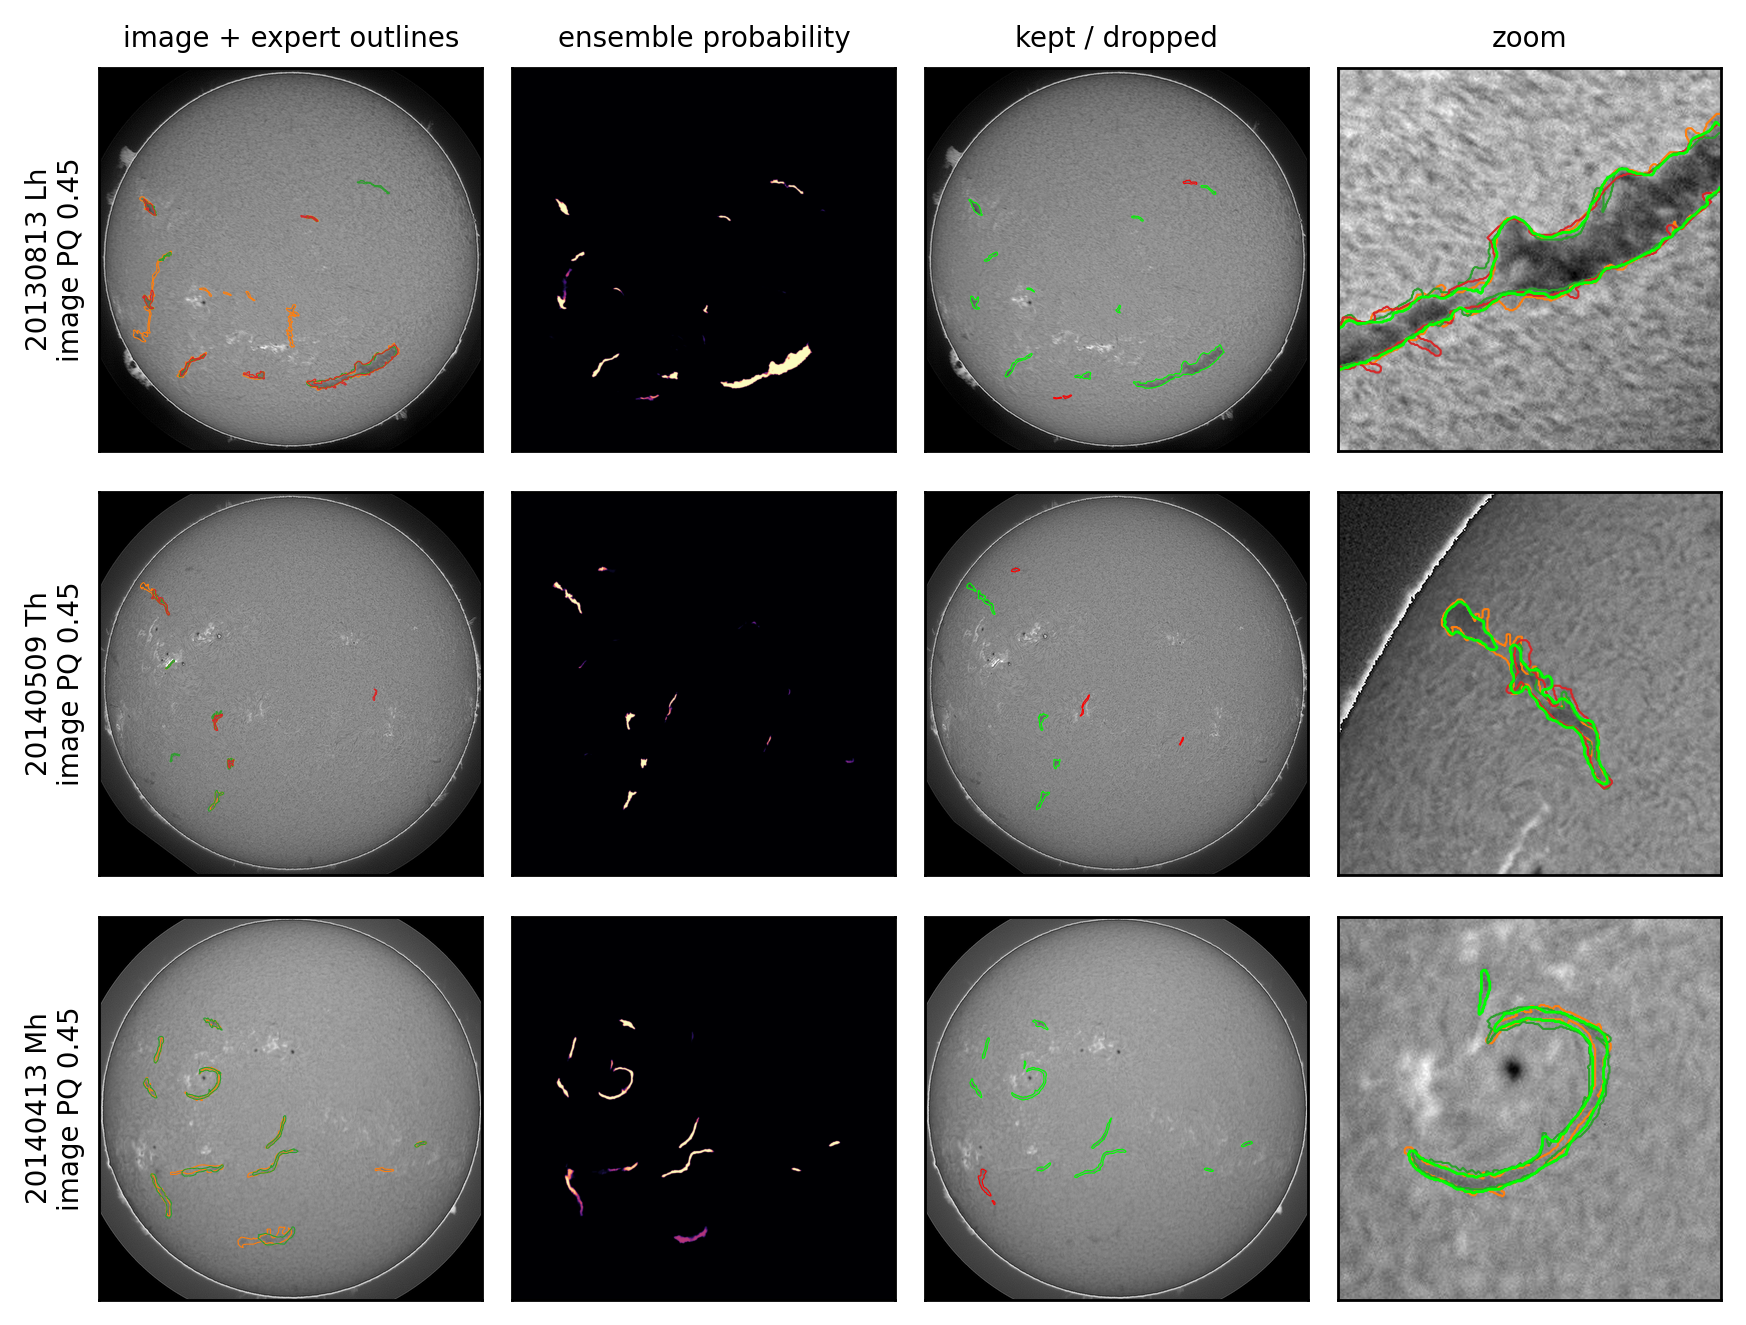
\includegraphics[width=0.9\textwidth]{figs/examples.png}
\caption{Out-of-fold segmentations of the training images whose PQ is closest to the median (one per site, at least two experts; not hand-picked). Column 1: the image with each expert's outlines in its own colour. Column 2: ensemble probability. Column 3: candidates kept (green) and dropped (red) by the keep rule. Column 4: zoom on the largest kept filament, experts' outlines and ours (green).}
\label{fig:examples}
\vspace{0.6em}
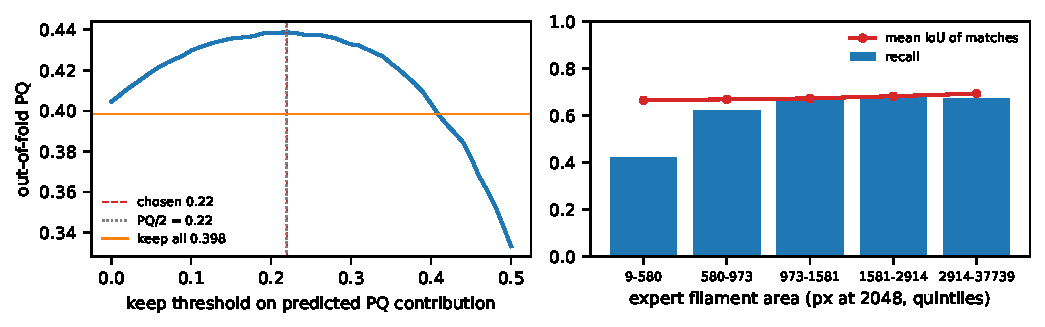
\includegraphics[width=0.8\textwidth]{figs/analysis.pdf}
\caption{Left: out-of-fold PQ against the keep threshold; the optimum coincides with PQ/2. Right: recall and IoU of matched filaments by expert filament area (quintiles).}
\label{fig:analysis}
\end{figure*}

% ==================================== %
%              EVALUATION              %
% ==================================== %
\section{Evaluation}\label{sec:evaluation}

\textbf{Strategy.} We validate on the 5 time-grouped folds (Sec.~\ref{sec:methodology}). Confidence intervals come from 2,000 bootstrap resamples of the 707 training images. The public leaderboard is reported only for the submitted variants, and it was not used to tune anything.

\begin{table}[t]
\caption{Out-of-fold PQ (95\% bootstrap CI over images) and public leaderboard. ``Area rule'': $p>0.5$, components $\ge$300~px.}
\label{tab:ablation}
\small
\begin{tabular}{lccc}
\toprule
Variant & PQ & SQ / RQ & Public \\
\midrule
Expert vs expert & 0.340 & 0.634 / 0.536 & -- \\
U-Net 1024, area rule & 0.404 & 0.673 / 0.600 & -- \\
U-Net 1024, keep rule & 0.432 & 0.675 / 0.640 & 0.37 \\
U-Net 1536, keep rule & 0.437 & 0.677 / 0.646 & -- \\
Ensemble, keep all & 0.398 {\scriptsize [0.389, 0.408]} & 0.674 / 0.591 & -- \\
\textbf{Ensemble, keep rule} & \textbf{0.439} {\scriptsize [0.429, 0.448]} & 0.678 / 0.647 & \textbf{0.39} \\
\bottomrule
\end{tabular}
\end{table}

\textbf{Results.} Table~\ref{tab:ablation} lists the variants and Figure~\ref{fig:examples} shows typical segmentations.
\begin{itemize}
    \item \textbf{Keep rule.} It adds $+0.040$ PQ over keeping every candidate (paired bootstrap CI $[0.036, 0.044]$). It removes half of the false positives (4,628 $\rightarrow$ 2,320) at the cost of 352 matches.
    \item \textbf{Threshold.} The out-of-fold optimum is at $\hat q=0.22$, the PQ/2 point the analysis predicts (Fig.~\ref{fig:analysis}, left).
    \item \textbf{Resolution and ensembling.} The 1536~px run gains over the 1024~px run through RQ more than SQ, and averaging the two adds a little more.
    \item \textbf{Stability.} Per fold, PQ ranges from 0.432 to 0.448 (mean 0.439, s.d.\ 0.007). Per site it ranges from 0.431 (Cerro Tololo, CI $[0.407, 0.452]$) to 0.451 (Udaipur, $[0.429, 0.476]$), with overlapping intervals.
    \item \textbf{Number of experts.} Images with one, two and three experts score 0.438, 0.454 and 0.429.
    \item \textbf{Leaderboard.} Out-of-fold gains carried over to the public leaderboard (0.37 $\rightarrow$ 0.39), but at a level about 0.05 lower, which suggests that the test images are harder or differently annotated.
\end{itemize}

\textbf{Strengths.}
\begin{itemize}
    \item The design follows from measured properties of the metric and the labels: consensus targets, full-resolution outlines, and a keep rule derived from the PQ break-even point.
    \item The model already agrees with the experts better than they agree with each other (0.439 vs 0.340).
    \item The scores are stable across folds, sites and expert counts.
    \item The pipeline is light: two networks, no instance head, and a small tabular model.
\end{itemize}

\textbf{Weaknesses.}
\begin{itemize}
    \item \textbf{Small filaments.} Recall falls to 0.42 for filaments below 580~px, against 0.62--0.68 for larger ones (Fig.~\ref{fig:analysis}, right). These are the faint, short structures experts disagree on most.
    \item \textbf{Outlines.} Matched outlines reach a mean IoU of only 0.67--0.69. Part of this is the experts' own outline spread (expert-vs-expert SQ 0.634).
    \item \textbf{Leaderboard gap.} The 0.05 gap between out-of-fold and public scores is not explained by our validation.
\end{itemize}

\textbf{Possible improvements.}
\begin{itemize}
    \item more diverse ensemble members (other encoders and seeds);
    \item sampling or loss weighting that favours small filaments;
    \item a per-candidate outline threshold chosen by a second learned model;
    \item modelling each expert's style, given the annotator identifiers in the data;
    \item self-training on unlabelled GONG frames.
\end{itemize}

% ==================================== %
%            ACKNOWLEDGMENT            %
% ==================================== %
\section{Acknowledgment}\label{sec:acknowledgment}
    % Do not change
    The organization of the Filament Segmentation Challenge 2026 is partially supported by the U.S. National Science Foundation (NSF) under Grant No. 2209912 and 2433781, directorate for Computer and Information Science and Engineering (CSE), and Office of Advanced Cyberinfrastructure (OAC), and Grant No. 2511630, AST Division Of Astronomical Sciences and MPS Directorate for Mathematical and Physical Sciences.

    The Filament Segmentation Challenge 2026 is sponsored by the U.S. National Science Foundation (NSF) National Solar Observatory (NSO).

    This work utilizes GONG data obtained by the NSO Integrated Synoptic Program, managed by the National Solar Observatory, which is operated by the Association of Universities for Research in Astronomy (AURA), Inc. under a cooperative agreement with the National Science Foundation and with contribution from the National Oceanic and Atmospheric Administration. The GONG network of instruments is hosted by the Big Bear Solar Observatory, High Altitude Observatory, Learmonth Solar Observatory, Udaipur Solar Observatory, Instituto de Astrofísica de Canarias, and Cerro Tololo Interamerican Observatory.

\bibliographystyle{ACM-Reference-Format}
\bibliography{main}

\end{document}
